\documentclass[11pt, oneside]{article}
\usepackage[letterpaper, margin=2cm]{geometry}
\usepackage{MATH566}
%\usepackage{sagetex}

\begin{document}
\noindent \textbf{\Large{Caleb Logemann \\
MATH 566 Discrete Optimization\\
Homework 7
}}

%\lstinputlisting[language=Sage]{03_2.sage}
\begin{enumerate}
  \item % #1
    A cut of $G$ is \emph{minimal} if there is no cut of $G$ properly contained
    in it.
    Prove that the random contraction algorithm returns only minimal cuts.

  \item % #2
    Implement Node Identification Minimum Cut Algorithm.
    Try it on the following graph:
    \begin{center}
      \tikzset{insep/.style={inner sep=2pt, outer sep=0pt, circle, fill},}
      \begin{tikzpicture}[scale=1.3]
        \draw
          (0,0) node[insep,label=below:$g$](g){}
          (2,0) node[insep,label=below:$f$](f){}
          (2,1) node[insep,label=right:$e$](e){}
          (2,2) node[insep,label=right:$a$](a){}
          (1,3) node[insep,label=above:$b$](b){}
          (0,1) node[insep,label=below left:$d$](d){}
          (0,2) node[insep,label=above:$c$](c){}
          (-1,1) node[insep,label=left:$h$](h){}
        ;
        \draw
          \foreach \x/\y/\t in {g/f/6, d/e/3, c/a/2, c/b/3, b/a/5,h/c/2, h/d/1}{
            (\x)--node[pos=0.5,label=above:$\t$]{} (\y)
          }
          (h)--node[pos=0.5,label=below:$5$]{} (g)
          \foreach \x/\y/\t in {g/d/2, d/c/4, f/e/2, e/a/3}{
            (\x)--node[pos=0.5,label=right:$\t$]{} (\y)
          }
        ;
      \end{tikzpicture}
    \end{center}

    I implemented the Node Identification algorithm with the following
    functions.
    \lstinputlisting[language=Sage]{nodeIdentification.sage}
    \lstinputlisting[language=Sage]{contractVertices.sage}

    The following script uses these function to run the Node Identification
    algorithm on the graph given for this problem.
    \lstinputlisting[language=Sage]{07_2.sage}

    The output of this script is

  \item % #3
    Implement Random Contraction Algorithm.
    Try it on the following graph. 
    Run it many times and based on your experiment conclude what is the probability that that your algorithm succeeds on this graph.
    \begin{center}
      \tikzset{insep/.style={inner sep=2pt, outer sep=0pt, circle, fill},}
      \begin{tikzpicture}[scale=1.3]
        \draw
          (0,0) node[insep,label=below:$g$](g){}
          (2,0) node[insep,label=below:$f$](f){}
          (2,1) node[insep,label=right:$e$](e){}
          (2,2) node[insep,label=right:$a$](a){}
          (1,3) node[insep,label=above:$b$](b){}
          (0,1) node[insep,label=below left:$d$](d){}
          (0,2) node[insep,label=above:$c$](c){}
          (-1,1) node[insep,label=left:$h$](h){}
        ;
        \draw
          \foreach \x/\y/\t in {g/f/6, d/e/3, c/a/2, c/b/3, b/a/5,h/c/2, h/d/1}{
            (\x)--node[pos=0.5,label=above:$\t$]{} (\y)
          }
          (h)--node[pos=0.5,label=below:$5$]{} (g)
          \foreach \x/\y/\t in {g/d/2, d/c/4, f/e/2, e/a/3}{
            (\x)--node[pos=0.5,label=right:$\t$]{} (\y)
          }
          ;
      \end{tikzpicture}
    \end{center}

    I implemented the random contraction algorithm with the following function.
    This function makes use of the contractVertices function, which was shown
    in the previous exercise, but is ommited here.
    \lstinputlisting[language=Sage]{randomContraction.sage}

    The following script uses these function to run the randomContraction
    algorithm on the graph given for this problem.
    \lstinputlisting[language=Sage]{07_3.sage}

  \item % #4
    Construct Gomory-Hu Tree for the following graph using the algorithm from the class. 
    Numbers on edges correspond to capacities.
    Show Show steps after every new cut.
    \begin{center}
      \tikzset{insep/.style={inner sep=2pt, outer sep=0pt, circle, fill},}
      \begin{tikzpicture}
        \draw
        \foreach \x/\a in {0/a,60/b,120/c,180/d,240/e,300/f}{
          (\x:2.5) node[insep](\a){}
        }
        (a) -- node[right]{1} (b) -- node[above]{3} (c) -- node[left]{2}
        (d) -- node[below]{1}(e) -- node[below]{3}(f) -- node[right]{1}(a)
        (b) -- node[below]{2} (d) -- node[below]{1} (f) -- node[right]{2} (b)
        ;
      \end{tikzpicture}
    \end{center}
    Check your answer with Sage using method \verb|Graph.gomory_hu_tree()|.
    Do not implement it yourself, just run it.

    First in order to run the Gomory Hu algorithm, I will label the vertices.
    \tikzstyle{vertex_style}=[circle, draw, inner sep=2pt]
    \tikzstyle{dot_style}=[circle, draw,fill=black,radius=0.002pt,inner sep=1pt]
    \begin{center}
      \begin{tikzpicture}[scale=1]
        \node[vertex_style](1) at (1.5,2) {$a$};
        \node[vertex_style](2) at (3.5,2) {$b$};
        \node[vertex_style](3) at (5,0) {$c$};
        \node[vertex_style](4) at (3.5,-2) {$d$};
        \node[vertex_style](5) at (1.5,-2) {$e$};
        \node[vertex_style](6) at (0,0) {$f$};

        \draw (1) --node[above]{$3$} (2);
        \draw (1) --node[above]{$2$} (6);
        \draw (2) --node[right]{$1$} (3) ;
        \draw (2) --node[right]{$2$} (4) ;
        \draw (2) --node[below]{$2$} (6) ;
        \draw (3) --node[below]{$1$} (4);
        \draw (4) --node[below]{$3$} (5);
        \draw (4) --node[above]{$1$} (6);
        \draw (5) --node[below]{$1$} (6);
      \end{tikzpicture}
    \end{center}

    First start with a tree that is $T = (\set{V}, \emptyset)$.
    This tree looks like.
    \begin{center}
      \begin{tikzpicture}
        \node[vertex_style] at (0, 0) {
          \begin{tikzpicture}
            \node[vertex_style](1) at (1.5,2) {$a$};
            \node[vertex_style](2) at (3.5,2) {$b$};
            \node[vertex_style](3) at (5,0) {$c$};
            \node[vertex_style](4) at (3.5,-2) {$d$};
            \node[vertex_style](5) at (1.5,-2) {$e$};
            \node[vertex_style](6) at (0,0) {$f$};

            \draw (1) --node[above]{$3$} (2);
            \draw (1) --node[above]{$2$} (6);
            \draw (2) --node[right]{$1$} (3) ;
            \draw (2) --node[right]{$2$} (4) ;
            \draw (2) --node[below]{$2$} (6) ;
            \draw (3) --node[below]{$1$} (4);
            \draw (4) --node[below]{$3$} (5);
            \draw (4) --node[above]{$1$} (6);
            \draw (5) --node[below]{$1$} (6);
          \end{tikzpicture}
        };
      \end{tikzpicture}
    \end{center}
    Now I will chose to find the minimum $a$-$b$ cut, which corresponds to
    finding the minimum $a$-$b$ flow in the following graph.
    The minimum cut found is shown in red.
    \begin{center}
      \begin{tikzpicture}[scale=1]
        \node[vertex_style](1) at (1.5,2) {$a$};
        \node[vertex_style](2) at (3.5,2) {$b$};
        \node[vertex_style](3) at (5,0) {$c$};
        \node[vertex_style](4) at (3.5,-2) {$d$};
        \node[vertex_style](5) at (1.5,-2) {$e$};
        \node[vertex_style](6) at (0,0) {$f$};

        \draw (1) --node[above]{$3$} (2);
        \draw (1) --node[above]{$2$} (6);
        \draw (2) --node[right]{$1$} (3) ;
        \draw (2) --node[right]{$2$} (4) ;
        \draw (2) --node[below]{$2$} (6) ;
        \draw (3) --node[below]{$1$} (4);
        \draw (4) --node[below]{$3$} (5);
        \draw (4) --node[above]{$1$} (6);
        \draw (5) --node[below]{$1$} (6);
        \draw[color=red,line width=1pt] (0,0.5)--(3.5,2.5);
      \end{tikzpicture}
    \end{center}
    Using this cut the new Gomory Hu tree is
    \begin{center}
      \begin{tikzpicture}
        \node[vertex_style](1) at (0, 0) {$a$};
        \node[vertex_style](X) at (5, 0) {
          \begin{tikzpicture}
            \node[vertex_style](2) at (3.5,2) {$b$};
            \node[vertex_style](3) at (5,0) {$c$};
            \node[vertex_style](4) at (3.5,-2) {$d$};
            \node[vertex_style](5) at (1.5,-2) {$e$};
            \node[vertex_style](6) at (0,0) {$f$};

            \draw (2) --node[right]{$1$} (3) ;
            \draw (2) --node[right]{$2$} (4) ;
            \draw (2) --node[below]{$2$} (6) ;
            \draw (3) --node[below]{$1$} (4);
            \draw (4) --node[below]{$3$} (5);
            \draw (4) --node[above]{$1$} (6);
            \draw (5) --node[below]{$1$} (6);
          \end{tikzpicture}
        };
        \draw (1)--node[above]{5}(X);
      \end{tikzpicture}
    \end{center}

    Now I will find the minimum $b$-$c$ cut in the following graph.
    The minimum cut found is shown in red.
    \begin{center}
      \begin{tikzpicture}[scale=1]
        \node[vertex_style](1) at (1.5,2) {$a$};
        \node[vertex_style](2) at (3.5,2) {$b$};
        \node[vertex_style](3) at (5,0) {$c$};
        \node[vertex_style](4) at (3.5,-2) {$d$};
        \node[vertex_style](5) at (1.5,-2) {$e$};
        \node[vertex_style](6) at (0,0) {$f$};

        \draw (1) --node[above]{$3$} (2);
        \draw (1) --node[above]{$2$} (6);
        \draw (2) --node[right]{$1$} (3) ;
        \draw (2) --node[right]{$2$} (4) ;
        \draw (2) --node[below]{$2$} (6) ;
        \draw (3) --node[below]{$1$} (4);
        \draw (4) --node[below]{$3$} (5);
        \draw (4) --node[above]{$1$} (6);
        \draw (5) --node[below]{$1$} (6);
        \draw[color=red,line width=1pt] (4,-2)--(4,2);
      \end{tikzpicture}
    \end{center}
    Using this cut the new Gomory Hu tree is
    \begin{center}
      \begin{tikzpicture}
        \node[vertex_style](a) at (0, 0) {$a$};
        \node[vertex_style](X) at (5, 0) {
          \begin{tikzpicture}
            \node[vertex_style](2) at (3.5,2) {$b$};
            \node[vertex_style](4) at (3.5,-2) {$d$};
            \node[vertex_style](5) at (1.5,-2) {$e$};
            \node[vertex_style](6) at (0,0) {$f$};

            \draw (2) --node[right]{$2$} (4) ;
            \draw (2) --node[below]{$2$} (6) ;
            \draw (4) --node[below]{$3$} (5);
            \draw (4) --node[above]{$1$} (6);
            \draw (5) --node[below]{$1$} (6);
          \end{tikzpicture}
        };
        \node[vertex_style](c) at (10, 0){$c$};
        \draw (a)--node[above]{5}(X);
        \draw (X)--node[above]{2}(c);
      \end{tikzpicture}
    \end{center}

    Now I will find the minimum $b$-$d$ cut in the following graph.
    The minimum cut found is shown in red.
    \begin{center}
      \begin{tikzpicture}[scale=1]
        \node[vertex_style](1) at (1.5,2) {$a$};
        \node[vertex_style](2) at (3.5,2) {$b$};
        \node[vertex_style](3) at (5,0) {$c$};
        \node[vertex_style](4) at (3.5,-2) {$d$};
        \node[vertex_style](5) at (1.5,-2) {$e$};
        \node[vertex_style](6) at (0,0) {$f$};

        \draw (1) --node[above]{$3$} (2);
        \draw (1) --node[above]{$2$} (6);
        \draw (2) --node[right]{$1$} (3) ;
        \draw (2) --node[right]{$2$} (4) ;
        \draw (2) --node[below]{$2$} (6) ;
        \draw (3) --node[below]{$1$} (4);
        \draw (4) --node[below]{$3$} (5);
        \draw (4) --node[above]{$1$} (6);
        \draw (5) --node[below]{$1$} (6);
        \draw[color=red,line width=1pt] (0,-1)--(5,-1);
      \end{tikzpicture}
    \end{center}
    Using this cut the new Gomory Hu tree is shown below.
    \begin{center}
      \begin{tikzpicture}
        \node[vertex_style](a) at (0, 0) {$a$};
        \node[vertex_style](X) at (5, 0) {
          \begin{tikzpicture}
            \node[vertex_style](2) at (1.75,1) {$b$};
            \node[vertex_style](6) at (0,0) {$f$};
            \draw (2) --node[below]{$2$} (6) ;
          \end{tikzpicture}
        };
        \node[vertex_style](Y) at (5, -5) {
          \begin{tikzpicture}
            \node[vertex_style](4) at (3.5,-2) {$d$};
            \node[vertex_style](5) at (1.5,-2) {$e$};
            \draw (4) --node[below]{$3$} (5);
          \end{tikzpicture}
        };
        \node[vertex_style](c) at (10, 0){$c$};
        \draw (a)--node[above]{5}(X);
        \draw (X)--node[above]{2}(c);
        \draw (X)--node[right]{5}(Y);
      \end{tikzpicture}
    \end{center}

    Now I will find the minimum $b$-$f$ cut in the following graph, where $e$
    and $d$ are contracted.
    \begin{center}
      \begin{tikzpicture}[scale=1]
        \node[vertex_style](1) at (1.5,2) {$a$};
        \node[vertex_style](2) at (3.5,2) {$b$};
        \node[vertex_style](3) at (5,0) {$c$};
        \node[vertex_style](4) at (2.5,-2) {$d,e$};
        \node[vertex_style](6) at (0,0) {$f$};

        \draw (1) --node[above]{$3$} (2);
        \draw (1) --node[above]{$2$} (6);
        \draw (2) --node[right]{$1$} (3) ;
        \draw (2) --node[right]{$2$} (4) ;
        \draw (2) --node[below]{$2$} (6) ;
        \draw (3) --node[below]{$1$} (4);
        \draw (4) --node[above]{$2$} (6);
        \draw[color=red, line width=1pt](1,2)--(1,-2);
      \end{tikzpicture}
    \end{center}
    Using this cut the new Gomory Hu graph is 
    \begin{center}
      \begin{tikzpicture}
        \node[vertex_style](a) at (1.5,2) {$a$};
        \node[vertex_style](b) at (3.5,2) {$b$};
        \node[vertex_style](c) at (5,0) {$c$};
        \node[vertex_style](f) at (0,0) {$f$};
        \node[vertex_style](X) at (2.5, -2) {
          \begin{tikzpicture}
            \node[vertex_style](4) at (3.5,-2) {$d$};
            \node[vertex_style](5) at (1.5,-2) {$e$};
            \draw (4) --node[below]{$3$} (5);
          \end{tikzpicture}
        };
        \draw (a)--node[above]{5}(b);
        \draw (b)--node[above]{2}(c);
        \draw (b)--node[above]{6}(f);
        \draw (b)--node[right]{5}(X);
      \end{tikzpicture}
    \end{center}

    Lastly I will find the minimum $d$-$e$ cut in the following contracted
    graph.
    \begin{center}
      \begin{tikzpicture}[scale=1]
        \node[vertex_style](1) at (2.5,0) {$a, b, c, f$};
        \node[vertex_style](4) at (3.5,-2) {$d$};
        \node[vertex_style](5) at (1.5,-2) {$e$};

        \draw (1) --node[right]{$4$} (4);
        \draw (1) --node[left]{$1$} (5);
        \draw (4) --node[below]{$3$} (5);
        \draw[color=red, line width=1pt] (1.3, -.5) -- (3.3, -2.5);
      \end{tikzpicture}
    \end{center}
    Thus the full Gomory Hu tree is
    \begin{center}
      \begin{tikzpicture}
        \node[vertex_style](a) at (1.5,2) {$a$};
        \node[vertex_style](b) at (3.5,2) {$b$};
        \node[vertex_style](c) at (5,0) {$c$};
        \node[vertex_style](d) at (3.5,-2) {$d$};
        \node[vertex_style](e) at (1.5,-2) {$e$};
        \node[vertex_style](f) at (0,0) {$f$};
        \draw (a)--node[above]{5}(b);
        \draw (b)--node[above]{2}(c);
        \draw (b)--node[above]{6}(f);
        \draw (b)--node[right]{5}(d);
        \draw (d)--node[below]{4}(e);
      \end{tikzpicture}
    \end{center}

    I checked this in Sage with the following script.
    \lstinputlisting[language=Sage]{07_4.sage}
    The output of this script is the following image of the Gomory Hu tree.
    \begin{center}
      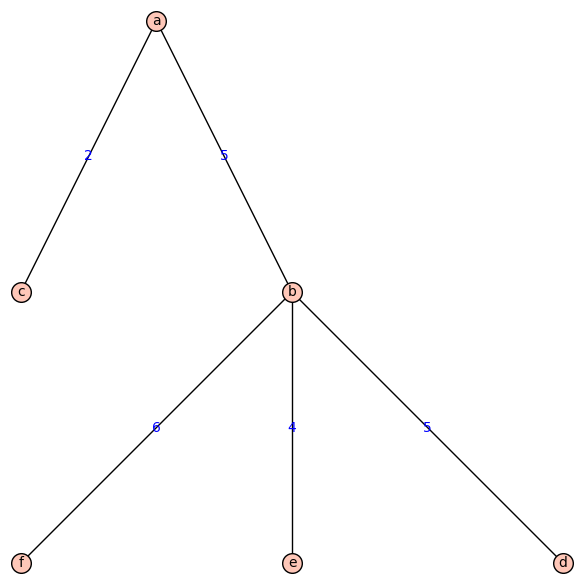
\includegraphics[scale=.8]{Figures/07_1.png}
    \end{center}
    This graph has a different structure but it has the same weights
    As the Gomory Hu tree is not unique I believe this confirms the
    tree that I arrived at.

\end{enumerate}
\end{document}
